\section{{Lecture 1 | Intro. to Reinforcement Learning}}

What makes reinfocement learning from other types of learning?
\begin{itemize}
\item There is no supervisor, only a reward signal
\item Feedback is delayed, not instantaneous.
\item Time really matters (sequential, non i.i.d data). Thus, breaks the fundamental assumption of supervised learning.
\item Agent's actions affect the subsequent data it receives. Thus, agent influences the data it receives.
\end{itemize}


Examples of reinforcement learning:
\begin{itemize}
    \item Fly stunt manoeuvres in a helicopter/ or control a robot.
    \item Play backgammon, chess, Go, Atari games.
    \item Manage investment portfolio.
    \item Manage a wind-farm/ power station.
\end{itemize}

\subsection{Elements of Reinforcement Learning --- Rewards}
\begin{itemize}
    \item A reward \(R_t\) is a scalar feedback signal.
    \item Indicates how well agent is doing at step \(t\).
    \item The agent's job is to maximise cumulative reward.
\end{itemize}
The reinforcement learning problem is to maximise the expected cumulative reward. The
reinforcement learning problem is based on the reward hypothesis.
\begin{definition}[Reward Hypothesis]
    All goals can be described by the maximisation of expected cumulative reward.
\end{definition}
Examples of rewards:
\begin{itemize}
    \item Fly stunt manoeuvres in a helicopter/ or control a robot.
    \begin{itemize}
        \item \(R_t = -1 \) for crash
        \item \(R_t = +1\) for following the desired trajectory
    \end{itemize}
    \item Play backgammon, chess, Go, Atari games.
    \begin{itemize}
        \item \(R_t = +1\) for winning the game
        \item \(R_t = 0\) for drawing the game
        \item \(R_t = -1\) for losing the game
    \end{itemize}
\end{itemize}

Sequential Decision Making:
\begin{itemize}
    \item Goal: select actions to maximise total future reward.
    \item Actions may have long term consequences.
    \item Reward may be delayed.
    \item It may be better to sacrifice immediate reward to gain more long-term reward.
    \item Thus, we need to consider the \textbf{whole sequence} of actions and rewards when making a decision.
    \item Examples:
    \begin{itemize}
        \item A financial investment --- may take years to mature.
        \item Refuelling a helicopter --- might prevent a crash in several hours.
        \item Move in chess --- may sacrifice a piece to get an opponent into a position in which they are more likely to lose.
    \end{itemize}
\end{itemize}
\subsection{Elements of Reinforcement Learning --- Agents and Environments}
\begin{figure}[H]
    \centering
    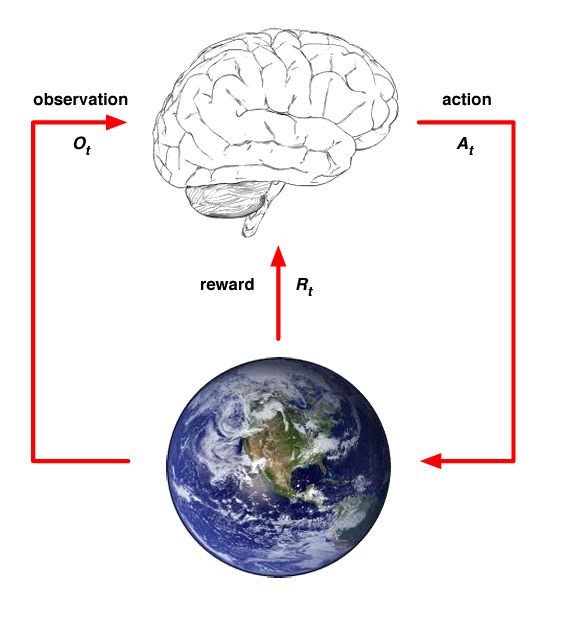
\includegraphics[width=0.60\textwidth]{figures/agent_world.png}
    \caption{Agent and Environment | The RL world loop.}
    \label{fig:agent_world}
\end{figure}

The interaction between the agnet and environments. The brain here represents 
the agent. The goal is to design and build this brain. The agent which take
the actions at each step, based on the information it is receiving from the
environment. The infomation that is coming is usually the observations
and the reward.
Thus, at each step we have for the agent:
\begin{itemize}
    \item The agent executes action \(A_t\).
    \item Receives observation \(O_t\).
    \item Receives scalar reward \(R_t\).
\end{itemize}
And for the environment:
\begin{itemize}
    \item Receives action \(A_t\).
    \item Emits observation \(O_{t+1}\).
    \item Emits scalar reward \(R_{t+1}\).
\end{itemize}

\subsection{Elements of Reinforcement Learning --- State}
\textbf{History and State:}
The history is the sequence of observations, actions, rewards:
\[
    H_t = A_1, O_1, R_1, \dots, A_t, O_t, R_t  
\]
This is practically all the observable variables to the agnet. The environment might have many more
such variables, but the agent does not have access to them. Thus such variables are irrelevant to the
algorithm that the agent will be based on. One of the examples can be the sensorimotor data stream
of the robot.
Ultimately, the agent's choice of action at any given time depends on the history. Thus, what
happens next depends on the history. 
But this history is not very useful. Typically this history is very long, and not practical to
use. Thus, we need to define a more useful quantity, the state.

\textbf{State:} is the information used to determine what happens next. It is the information that is
relevant to make the decision. It is a function of the history:
\[
    S_t = f(H_t)
\]
One of the valid definitions of the state is the complete history, or just the last observation. 
In Atari games, the state is the usually the last 4 frames of the game.

Here we are describing 3 different definations of the state:\\
\textbf{Environment State: }
\begin{itemize}
    \item The environment state \(S_t^e\) is the environment's private representation.
    \item whatever the environment uses to pick the next observation and reward. 
    \item The environment state is usually not visible to the agent.
    \item Even if \(S_t^e\) is visible, it may not be useful and might contain irrelevant information.
\end{itemize}
\textbf{Agent State:}
\begin{itemize}
    \item The agent state \(S_t^a\) is the agent's internal representation.
    \item whatever information the agent uses to pick the next action.
    \item it is the information used by the reinforcement learning algorithms.
    \item It can be any function of the history:
    \[
        S_t^a = f(H_t)  
    \]
\end{itemize}
\textbf{Information State:}\\
An information state (also called Markov state) contains all useful information from the history.
\begin{definition}[Markov State]
    A state \(S_t\) is Markov if and only if:
    \[
        \mathbb{P} [S_{t+1} | S_t] = \mathbb{P} [S_{t+1} | S_1, \dots, S_t]  
    \]
\end{definition}
In other words, the future is independent of the past given the present.
\[
    H_{1:t} \to S_t \to H_{t+1:\infty}
\]
Thus, the state is a sufficient statistic of the future. And hence once the state is known, the history
may be thrown away. The state captures all useful information from the history.
For example, the markov state for the helicopter is the position, velocity, and orientation, and the
angular velocity, and any other external disturbances. Once, these states are known, the next 
state can be predicted, without needing any other information from the history.

Also note that, the environment state \(S_t^e\) is Markov. Also, one of the rather not useful Markov
state is the complete history \(H_t\).\\
\begin{example}[Rat Example]
\begin{figure}[H]
    \centering
    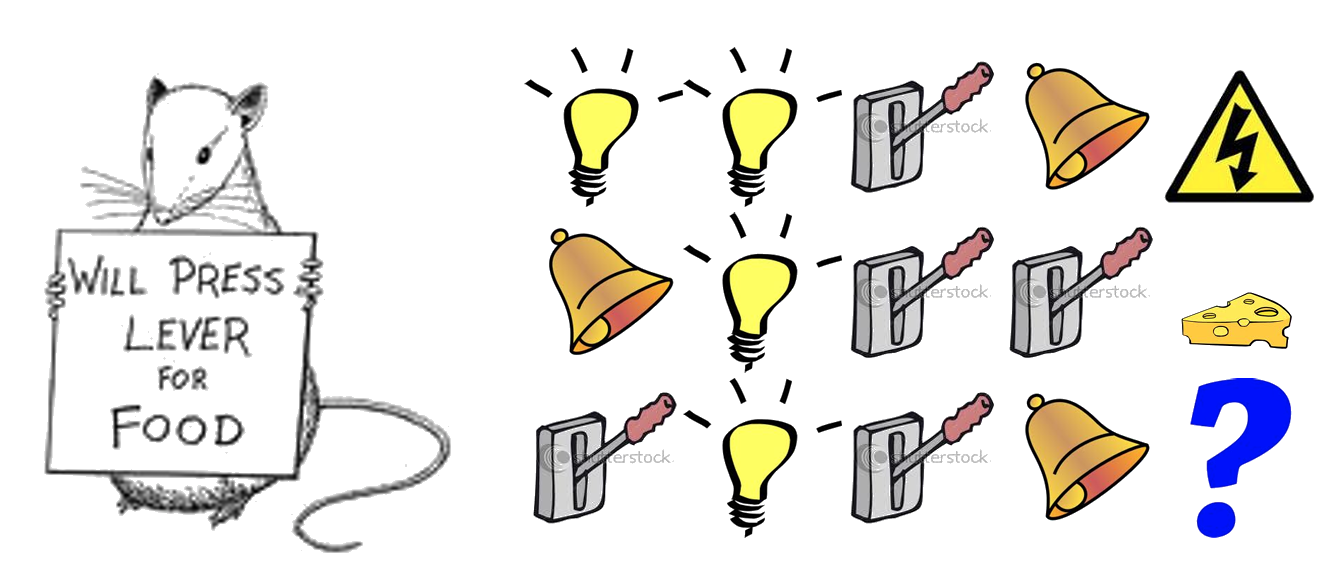
\includegraphics[width=0.8\textwidth]{figures/rat_example.png}
    \caption{Action and Reward sequence/ history for the rat example.}
    \label{fig:rat_example}
\end{figure}
Based on the history and expericence of the rat sequence, shown 
in \autoref{fig:rat_example}, we can define the state as:
the rat can either be electrocuted or be rewarded with a piece of cheese. Now is
we are using the last three observations in the sequence, as the agent state, 
then we would believe that the rat might be electrocuted, but if we use the
agent state as the count for lights, bells and levers, then we would expect the cheese would be 
rewarded. 

Thus, it clear that what we believe will happen next, depends on our representation of the state.
Another example of the valid state would be to consider the entire history as the state.
From this state representation, we don't know what will happen next.
\end{example}
So the state representation defines what happens next, which can be characterised by many different
ways, and it is up to the designer to choose the state representation to be useful to solve the 
problem at hand.

\textbf{Environments:}\\
Fully observable environments: the agent directly observes the environment state.
\[
    \implies O_t = S_t^a = S_t^e
\]
Meaning that the agent state and the environment state are the same.\\
Formally, this representation is called as a \textbf{Markov Decision Process (MDP)}.\\
Partially observable environments: the agent indirectly observes the environment state.
Examples:
\begin{itemize}
    \item A robot with a camera vision isn't told its exact position.
    \item A trading agent only observes current price and volume.
    \item A poker agent only observes public cards and bets.
\end{itemize}
Now the agent state and the environment state are different.
\[
    \implies S_t^a \neq S_t^e  
\]
Formally, this representation is called as a \textbf{Partially Observable Markov 
Decision Process (POMDP)}. Thus, the agent must construct its own state representation \(S_t^a\).
Some examples of the agent state representation:
\begin{itemize}
    \item Complete history \(H_t\).
    \item Beliefs about the environment state: \(S_t^a = (\mathbb{P}[S_t^e = s^1], 
    \dots, \mathbb{P}[S_t^e = s^n])\) i.e. that there is some probability that the environment
    state is \(s^1\), and some probability that the environment state is \(s^2\), and so on.
    \item Recurrent neural network: \(S_t^a = \sigma (S_{t-1}^a W_s + O_t W_o)\).
\end{itemize}

\subsection{Inside an RL Agent}
An RL agent may include one or more of the following:
\begin{itemize}
    \item \textbf{Policy}: agent's behaviour function.
    \item \textbf{Value function}: how good is each state and/or action.
    \item \textbf{Model}: agent's representation of the environment.
\end{itemize}

\textbf{Policy}:\\
Policy in short is the behaviour of the agent. It is the agent's behaviour function. Thus, 
it is a map from state to action. It can be:
\begin{itemize}
    \item deterministic policy: \(a = \pi(s)\)
    \item stochastic policy: \(\pi(a|s) = \mathbb{P}[A_t = a | S_t = s]\)
\end{itemize}

\textbf{Value Function:}\\
The value function is the expected total future reward. This is used 
to evaluate the goodness/badness of states. It is the expected total future reward from state \(s\).
\[
    v_\pi(s) = \mathbb{E}_\pi [R_t + \gamma R_{t+1} + \gamma^2 R_{t+2} + \dots | S_t = s]  
\]
where, \(\gamma \in [0, 1]\) is called the discount factor, which determines how much importance
is given to the immediate reward, compared to the future rewards.\\

\textbf{Model:}\\
The model predicts what the environment will do next. The idea is do predict what the next state
will be based on the environment, and plan accordingly to maximise the reward. This is often 
characterised into two parts:
\begin{itemize}
    \item \textbf{Transition model}: \(\mathcal{P} \) predicts the next state (or states) given
     current state and action.
    Can be considered as the dynamics of the environment.
    \[
        \mathcal{P}_{ss'}^a = \mathbb{P}[S_{t+1} = s' | S_t = s, A_t = a]
    \]
    \item \textbf{Reward model}: \(\mathcal{R}\) predicts the next immediate reward given
     current state and action.
    \[
        \mathcal{R}_s^a = \mathbb{E}[R_{t+1} | S_t = s, A_t = a]
    \]
\end{itemize}

It is not necessary to have a model to solve the reinforcement learning problem. 

\begin{example}[Maze Example]
    One of the standard RL grid world examples. The goal is to go from the 
    start state to the goal state. The agent can move in any of the four directions,
    i.e. up, down, left, right. The agent receives a reward of -1 for each step it takes.
    Thus, the agent wants to reach the goal state in as few steps as possible.
    % create a figure for the maze examplw with subfigures to denote policy and
    % value function. there should be 3 images alonside each other
    \begin{figure}[H]
        \centering
        \begin{subfigure}[b]{0.3\textwidth}
            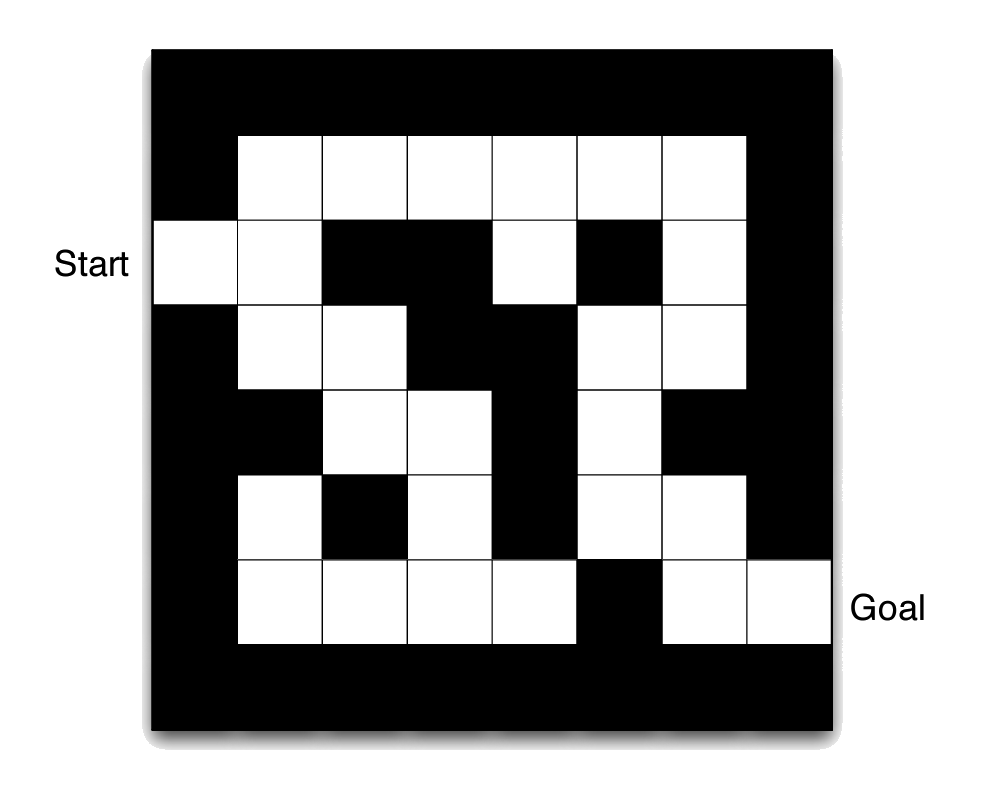
\includegraphics[width=\textwidth]{figures/maze_blank.png}
            \caption{Maze Example}
            \label{fig:maze_example}
        \end{subfigure}
        \begin{subfigure}[b]{0.3\textwidth}
            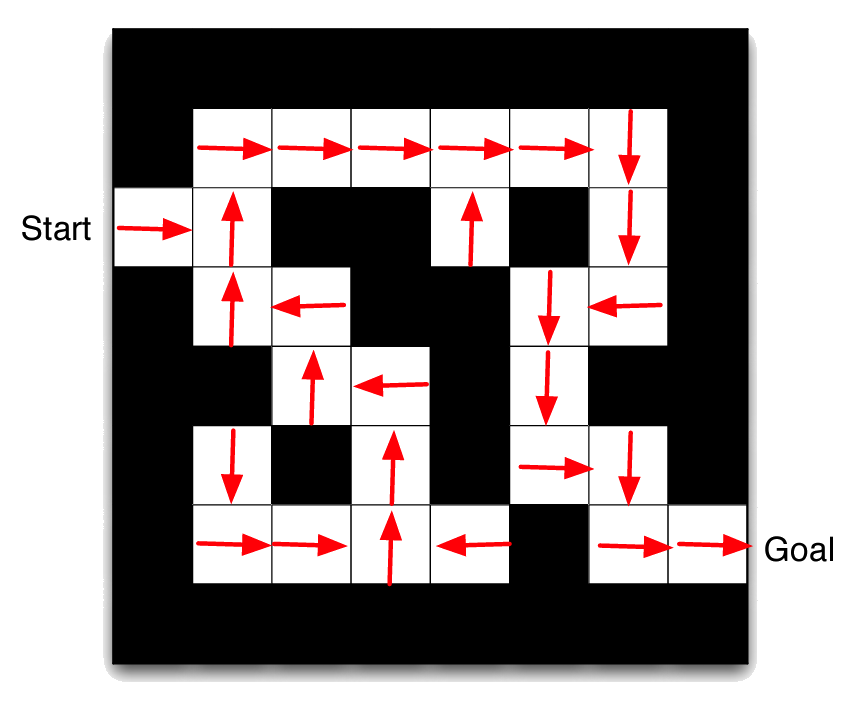
\includegraphics[width=\textwidth]{figures/maze_policy.png}
            \caption{Policy}
            \label{fig:maze_policy}
        \end{subfigure}
        \begin{subfigure}[b]{0.3\textwidth}
            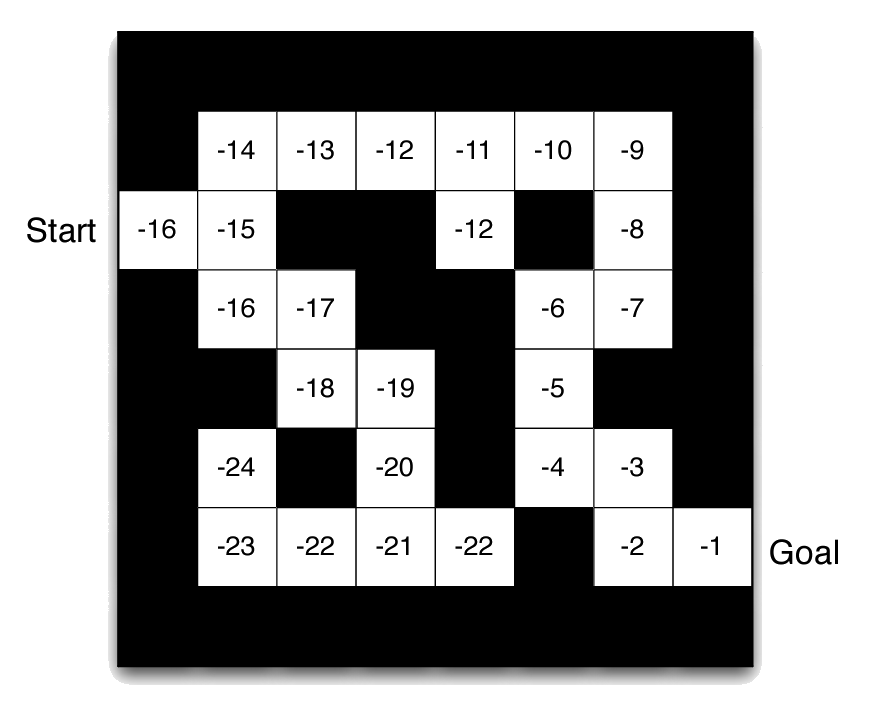
\includegraphics[width=\textwidth]{figures/maze_value.png}
            \caption{Value Function}
            \label{fig:maze_value_function}
        \end{subfigure}
        \caption{Maze Example}
    \end{figure}

    The arrows in the \autoref{fig:maze_policy} denote the policy
    \(\pi (s)\) of the agent for each state \(s\)  So the agent will transition from ome state to another based on
    the direction of the arrow provided by the policy. In this case it is a 
    deterministic policy, that directly maps the state to the action.\\
    The value function in this example is the number of steps 
    it takes to reach the goal state.
    Now once we have all the values, it is very simple to build an optimal policy. 

\end{example}

So to categorise the RL agents:
\begin{itemize}
    \item Value based agents: select actions based on value functions.
    \item Policy based agents: select actions based on policy functions.
    \item Actor-critic agents: select actions based on both value and policy functions.
\end{itemize}
Based on the model:
\begin{itemize}
    \item Model free agents: do not have a model/ or explicitly build the model of the environment.
    \item Model based agents: have a model of the environment.
\end{itemize}
Both, model based an model free agents can be value based, policy based, or actor-critic agents.

\subsection{Problems within Reinforcement Learning}
\subsubsection{RL and Planning}
There are two main problems in sequential decision making:
\begin{itemize}
    \item \textbf{Reinforcement Learning:}
    \begin{itemize}
        \item The environment is initially unknown.
        \item The agent interacts with the environment.
        \item The agent improves its policy.   
    \end{itemize}
    \item \textbf{Planning:}
    \begin{itemize}
        \item A model of the environment is known.
        \item The agent performs computations with its model (without any external interaction).
        \item The agent improves its policy.
        \item thus the policy does reasoning, introspection, search etc.
    \end{itemize}
\end{itemize}
These two approaches are linked. First, we can learn a model of the environment, and then use 
planning approach to improve the policy.
This can be understood from the Atari game example.
\begin{figure}[H]
    \centering
    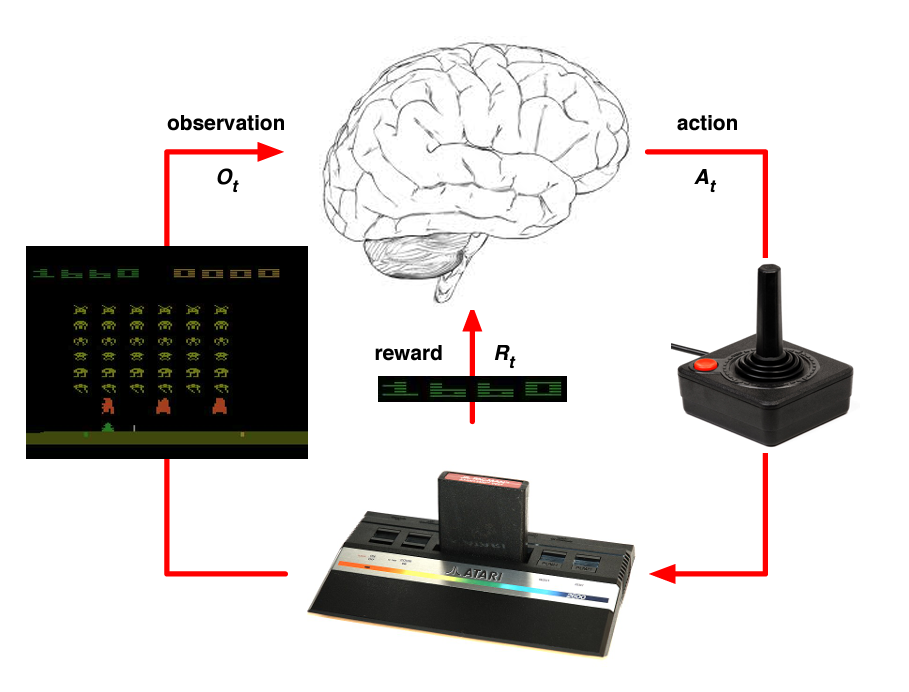
\includegraphics[width=0.8\textwidth]{figures/atari_rl.png}
    \caption{Atari Game Example --- RL}
    \label{fig:atari_rl}
\end{figure}
The \autoref{fig:atari_rl} shows 
the RL approach to the Atari game. The rules of the game are unknown, 
and the agent learns from the interaction with the game. The loop is basically
pick actions on the joystick, see pixels and scores.

\begin{figure}[!htp]
    \centering
    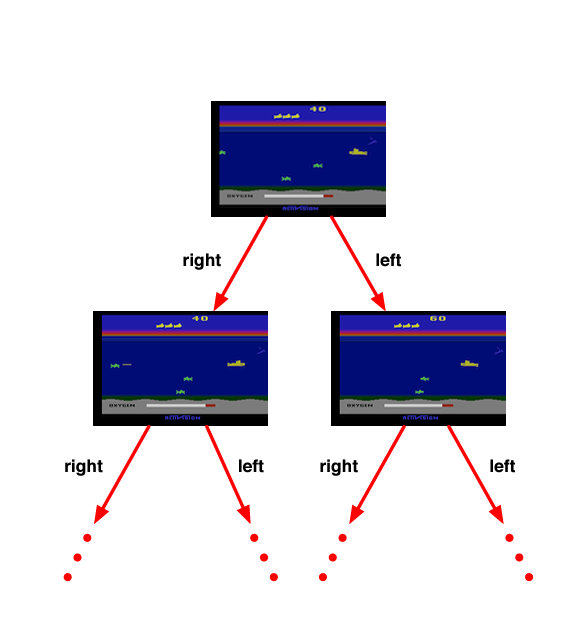
\includegraphics[width=0.6\textwidth]{figures/atari_planning.png}
    \caption{Atari Game Example --- Planning}
    \label{fig:atari_planning}
\end{figure}
The \autoref{fig:atari_planning} shows the planning approach to the Atari game. 
The rules of the game are known, and the agent can query the emulator, thus 
giving the perfect model inside the agent's brain. So the agent has 
perfect answer to the question, which state \(s_t\) the agent will be in, if it takes
action \(a_t\) in state \(s_{t-1}\), and the corresponding reward \(r_t\).
Thus, the agent can plan ahead, and find the optimal policy.

\subsubsection{Exploration and Exploitation}
Reinformcement learning is like trial and error learning. The agent should try to maximise the
reward, but it does not know what will happen next. Thus, the agent must figure out the 
best part of the state-action space, from its experience of the environment, without
losing too much reward along the way, while it is learning.\\

Thus, the exploration and exploitation trade-off is a fundamental dilemma in reinforcement learning.
\begin{itemize}
    \item \textbf{Exploration:} gaining more information about the environment.
    \item \textbf{Exploitation:} exploiting known information to maximise reward.
\end{itemize}